\documentclass[a4paper,11pt]{article}

% set up sensible margins (same as for cssethesis)
\usepackage[paper=a4paper,left=30mm,right=30mm,top=25mm,bottom=25mm]{geometry}
\usepackage{natbib} % Use the natbib bibliography and citation package
\usepackage{setspace} % This is used in the title page
\usepackage{graphicx} % This is used to load the crest in the title page
\usepackage{physics} % Used for \abs

% non-template packages
\usepackage{paralist}
\usepackage{multicol}
\usepackage{caption}
\usepackage{tabularx, booktabs}
\newcolumntype{Y}{>{\centering\arraybackslash}X}
\usepackage{listings}
\lstset{
	numbers=left, 
	numberstyle=\small, 
	numbersep=8pt, 
	frame = single, 
	language=Python, 
	framexleftmargin=17pt}

\usepackage{tikz}
\usepackage{smartdiagram}

\usepackage[font={small,it}]{caption}
\usepackage{hyperref}
\usepackage{xcolor}
\usepackage{lscape}
\hypersetup{
	colorlinks,
	linkcolor=teal,
	citecolor=teal,
	urlcolor=blue
}

\usepackage[english]{babel}
\usepackage{blindtext}
\usepackage{footnote}
%\makesavenoteenv{tabular}
%\makesavenoteenv{table}

%tikz stuff
\usepackage{tikz}
\usetikzlibrary{shapes, arrows, trees}
\tikzstyle{decision} = [diamond, draw, fill=green!20, text width=4.5em, text badly centered, node distance=3cm, inner sep=0pt]
\tikzstyle{block} = [rectangle, draw, fill=yellow!20, text width=3cm, text centered, rounded corners, minimum height=4em]
\tikzstyle{line} = [draw, -latex']
\tikzstyle{straight} = [draw]


\usepackage{array}
\newcolumntype{L}[1]{>{\raggedright\let\newline\\\arraybackslash\hspace{0pt}}m{#1}}
\newcolumntype{C}[1]{>{\centering\let\newline\\\arraybackslash\hspace{0pt}}m{#1}}
\newcolumntype{R}[1]{>{\raggedleft\let\newline\\\arraybackslash\hspace{0pt}}m{#1}}

\usepackage{float}

%\hypersetup{
%	colorlinks,
%	linkcolor={red!50!black},
%	citecolor={blue!50!black},
%	urlcolor={blue!80!black}
%}

\begin{document}
	
% Set up a title page
\thispagestyle{empty} % no page number on very first page
% Use roman numerals for page numbers initially
\renewcommand{\thepage}{\roman{page}}

\begin{spacing}{1.5}
	\begin{center}
		{\Large \bfseries
			School of Computer Science (BICA) \\
			Monash University}
		
		
		\vspace*{30mm}
		
		
\includegraphics[width=5cm]{graphics/MonashCrest.pdf}
		
		\vspace*{15mm}
		
		{\large \bfseries
			Literature Review, 2017
		}
		
		\vspace*{10mm}
		
		{\LARGE \bfseries
			Review of optimal multi-agent Pathfinding algorithms and usage in warehouse automation
		}
		
		\vspace*{20mm}
		
		{\large \bfseries
			Phillip Wong
			
			\vspace*{20mm}
			
			
			Supervisors: \parbox[t]{50mm}{Daniel Harabor,\\Pierre Le Bodic}
		}
		
	\end{center}
\end{spacing}

\newpage

\tableofcontents

\newpage
% Now reset page number counter,and switch to arabic numerals for remaining
% page numbers 
\setcounter{page}{1}
\renewcommand{\thepage}{\arabic{page}}

\section{Introduction} \label{sec:introduction}
% What
The order picking process is the number one expense in the operating cost of warehouse systems (\cite{de2007design}). Order picking involves the retrieval of inventory from around the warehouse.
This project looks at the use of multi-agent pathfinding (MAPF) within order picking. In particular, we will be exploring Kiva systems (\cite{wurman2008coordinating}) where the order-picking process is performed by automated vehicles. 

Firstly we define the components making up a Kiva system (Figure~\ref{fig:kivaprocess}). \textit{Drive units} are our autonomous vehicles which move around the warehouse, retrieving and delivering shelving units. These shelving units are known as \textit{storage pods} which are usually organized in aisles. Lastly we have the \textit{picking station} where a human workers are situated. So the process of order picking within a Kiva system is as follows:
\begin{compactenum}
	\item An order is received requesting one or more products
	\item The system identifies storage pod shelves containing the said products
	\item The system schedules drive units agent to pickup the storage pods
	\item Once ready, the drive unit agent will move to the storage pod, pick it up and deliver it to the correct picking station
	\item Once the drive unit has delivered the storage pod, a human worker situated at the picking station will pick the product off the storage pod and pack it into a box
	\item After the storage pod has been picked, the drive unit agent returns it to a suitable location
	\item Finally once all the products for the order have been picked and packed, the box it is processed and sent off
\end{compactenum}

\noindent As this process describes, Kiva systems have more hard problems to solve than MAPF. Scheduling occurs when these drive unit agents run out of battery or the storage pods run low on products. Both of these have to be replenished, hence a schedule needs to be determined. Another example is the robotics challenge described in the Amazon picking challenge (\cite{correll2016lessons}). The motivation of this challenge is replace the human worker with a robotic arm to perform the picking and packing and hence improve the reliability and speed of picking. 

Solving all these problems and applying them in one solution has been done by the creators of Kiva systems but is unfortunately is not described in any literature. The consequences of optimizing these systems together would be very useful to see what has the most effect but is out of the scope of this project.

So looking at the role of MAPF, we see that the MAPF problem occurs when the drive unit agent retrieves, delivers or returns the storage pods. Here we need a solution to coordinate drive unit agents so they can move around the warehouse without colliding with other agents. We can conclude that Kiva systems in production are using a suboptimal algorithms as these warehouses run over 1000 agents but solving MAPF optimally is an NP-hard problem (\cite{yu2013structure}). This forms the motivation behind our project, to look at the benefits we may find in Kiva systems by using an optimal approach and what we will sacrifice for scalability.

Ultimately the contributions of this literature review is in the comparison between optimal and suboptimal MAPF algorithms. We identify algorithms which have been applied to a Kiva systems setting and what conclusions they have drawn. Additionally we outline how optimal algorithms have tried improve scalability.

\begin{figure}[h!]
	\centering
	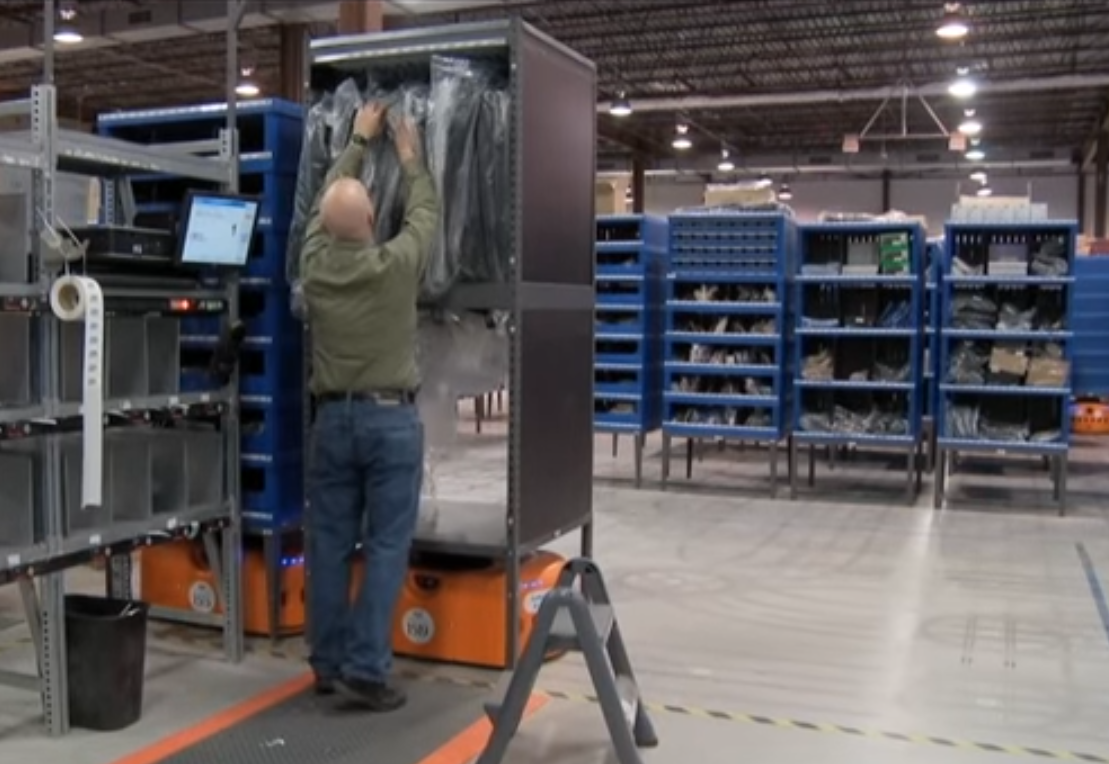
\includegraphics[width=0.6\textwidth ]{graphics/kivaprocess}
	\caption{A worker picking an order from a storage pod. The orange robot underneath is the drive unit. (\cite{kivayoutube2010quietlogistics})}
	\label{fig:kivaprocess}
\end{figure}

% How
Section~\ref{sec:background} describes in detail the MAPF problem and according terminology. Section~\ref{sec:suboptimal} describes some state-of-the-art suboptimal MAPF algorithms focusing on the scalability. Section~\ref{sec:optimal} looks at optimal MAPF algorithms. Section~\ref{sec:generalimprovements} looks at two techniques which can be applied to most MAPF algorithms and has substantial improvements. Finally Section~\ref{sec:discussion} compares suboptimal and optimal algorithms with a focus on putting them into the context of a Kiva system environment.

%In order to find an optimal solution we will be using formulating the MAPF problem as a mixed integer program. Section~\ref{sec:optimal} will look at past approaches taken to MAPF.
% Why
%The aim of this literature review is to summarize the state-of-the-art in optimal MAPF, compare them to the scalability of suboptimal algorithms and identify which algorithms have been tested in a Kiva system environment.

\section{Background} \label{sec:background}
\subsection{Single-agent pathfinding} The single-agent pathfinding problem aims to find a path from start node to goal node. A detailed review of single agent search algorithms can be found in the \textit{grid-based path planning competition} (\cite{sturtevant2015grid}). The paper overviews all the entries to the competition and their relative performance. The algorithms are run on a number of game maps from \cite{sturtevant2012benchmarks} which are used for benchmarking and these maps are used in many MAPF benchmarks. These results from \cite{sturtevant2015grid} are a few years old but we are expecting new approaches from this year's GPPC.

In this project, we aim to look at two single-agent search algorithms: \textit{jump point search} (\cite{harabor2011online}) and \textit{compressed path databases} (\cite{strasser2015compressing}). \cite{botea2013pathfinding} outlines both these algorithms as other single-agent search techniques in the context of computer games.

\subsection{Multi-agent pathfinding} Here we briefly describe the general problem of MAPF, in Section~\ref{sec:problemdef} we will formally define the problem in the context of Kiva systems as well as outlining terminology. The task of the MAPF problem is to coordinate multiple agents moving around an environment. Each agent is a goal location and the algorithm is required to find a path for each agent while ensuring that agent collides with another. A common secondary objective is to minimize either the makespan of the system or the sum of individual costs (SIC). As mentioned in Section~\ref{sec:introduction}, solving MAPF optimally is an NP-hard problem (\cite{yu2013structure}). Suboptimal and optimal MAPF have vastly different properties in scalability and solution quality. Thus they are compared in different sections [\ref{sec:optimal}, \ref{sec:suboptimal}]. Below are some important properties of MAPF algorithms. Table~\ref{table:comparison} shows a comparison of these properties across the MAPF algorithms discussed in this literature review.

\noindent \textbf{Completeness:} the algorithm will return valid solution to the MAPF problem if one exists

\noindent \textbf{Solution quality:} solution quality is usually measured as the objective of makespan or sum of individual costs (SIC). Makespan is the number of timestep required from the start state to the goal state where all agents are at their goals. SIC is the sum of the number of timesteps taken for each individual agent to reach their goal.
\begin{compactitem}
	\item Optimal: finds the optimal path to the goal minimizing the objective
	\item Bounded suboptimal: given a optimal path cost of $C$, the cost of a bounded suboptimal solution, $B$ is guaranteed to be within $C$ and $w*C$ where $w$ is a user set parameter. Hence, $C \le B \le wC$.
	\item Suboptimal: finds a path to the goal with no guarantee of solution cost
\end{compactitem}

\noindent \textbf{Anonymous:} In an anonymous MAPF problem the goal location is interchangeable and any agent can be assigned to a goal in order to satisfy the MAPF problem.

\noindent \textbf{Anytime:} The search can spend more computation to improve the solution quality or number of solutions. It can stop earlier at any time and return a path.

\noindent \textbf{Centralized / Coupled:} A centralized algorithm looks at all agents together in planning paths, whereas in a decentralized algorithm, paths are found for one agent at time. A centralized approach is usually used in finding an optimal solution but is not scalable. Accordingly a decentralized approach scales up to many agents but is suboptimal and often non-complete.

\subsection{Bounded-suboptimal variants} 
A bounded suboptimal variant is a variant of an optimal MAPF algorithm. The defining feature of a bounded suboptimal variant is that we are able to guarantee that the cost of the bounded suboptimal solution, $B$ lies within the optimal cost $C$ and $w*C$ where $w$ is a user-defined parameter. A bounded suboptimal variant provides a way of trading speed for solution quality and is especially relevant this project as we want to find a middle ground between optimality and speed for Kiva systems. The optimal algorithms in \ref{sec:optimal} will mention any bounded suboptimal variants if they exist.

\noindent \textbf{Integer Linear Programming}. Integer Linear Programming (ILP) is an optimization technique. It looks at an objective function subject to a list of constraints and finds the optimal solution for each variable. \textbf{not sure what to write here?}

%\[C \le B \le w*C\]
%
%Our project is aiming to make a bounded suboptimal variant of our algorithm due to the large-scale of the simulation (Section~\ref{sec:background}). By adjusting $w$ we are able to relax the problem and find a solution faster at the loss of solution quality.

\subsection{Problem definition} \label{sec:problemdef}
This section will formally define the MAPF problem in the context of Kiva Systems. The goal of MAPF is to coordinate agents and find a path for each agent to their goal while ensuring that no path conflicts. Here, a path is a sequence of actions, where an action is one of $\{up, down, left, right, wait\}$. A path is said to conflict with another when on the same timestep: two agents share the same node or two agents cross the same edge.

The warehouse environment is modelled as a square grid map in order to reduce the complexity of the MAPF algorithm. This is a  Graph $G(V, E)$ where $V$ is the set of nodes on the grid map and $E$ is the set of edges between nodes. On this map we have the components of a Kiva system: storage pods, drive units and picking stations (Figure~\ref{fig:kivawarehouse}), hence these are:
\begin{compactitem}
	\item A set of picking stations, $P$, where for all $p \in P$, $location (p) \in V$
	\item A set of storage pods, $S$, where for all $s \in S$, $location (s) \in V$
	\item A set of drive units, $K$, where for all $k \in K$, $location(k) \in V$ and $goal(k) \in V$
\end{compactitem}

\noindent Collision occurs between a drive unit and a storage pod iff a drive unit is carrying a storage pod. In other words, drive units are capable of maneuvering underneath storage pods. Additionally collision always occurs between drive units, picking stations and other drive units.

\begin{figure}[h]
	\centering
	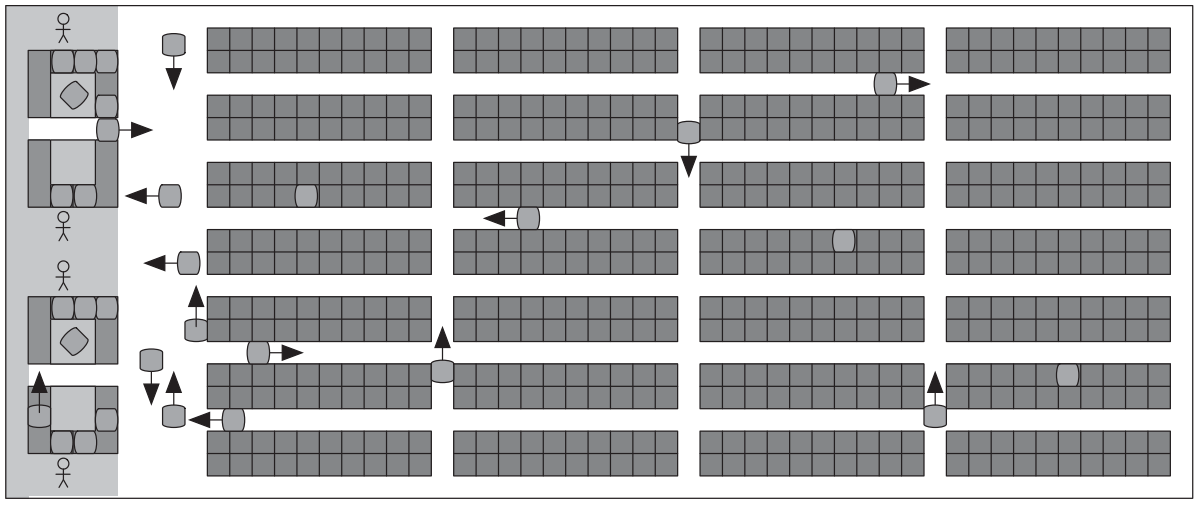
\includegraphics[width=0.9\textwidth]{graphics/kivasystemlayout}
	\caption{Kiva system represented on an orthagonal grid map (\cite{wurman2008coordinating})}
	\label{fig:kivawarehouse}
\end{figure}

Different to traditional the MAPF problem, the objective of a Kiva system is to minimize the down-time of human pickers. Kiva systems run 24 hours a day hence the Makespan and SIC are not quite representative as they require a goal-state. For MAPF algorithms which were applied to Kiva systems, we look at whether new objectives were used to measure performance.

\section{Suboptimal multi-agent pathfinding algorithms} \label{sec:suboptimal}
Suboptimal MAPF algorithms usually use a decentralized approach\footnote{decentralized is also known as decoupled}. In a decoupled approach, paths are found for one agent at time as oppose to a coupled approach which looks at all agents globally. These algorithms usually have the properties of being suboptimal and incomplete.

%\begin{center}
%\begin{tikzpicture}
%\centering
%\draw[step=1cm,gray,very thin] (0,0) grid (5,3);
%\fill[gray!] (0,0) rectangle (3,1);
%\node at (0.5, 2.5) {$a_2$};
%\node at (0.5, 1.5) {$a_1$};
%\end{tikzpicture}
%\end{center}

\subsection{Cooperative A*}
Cooperative A*
Exponential in number of agents

\cite{holte1995hierarchical}

\cite{silver2005cooperative} gives an overview of these three algorithms.

%\subsection{FAR}
%Flow Annotation Replanning (FAR) (Wang and Botea 2008) imposes unidirectional travel on top of an initially undirected gridmap. The travel direction alternates across the rows (and columns), covering the grid with criss- crossing virtual “road lanes”. Topology-specific additional rules, applied locally, preserve the connectivity across the map. In terms of map abstraction, this boils down to remov- ing some directed edges from a graph, as opposed to splitting a map into subgraphs. FAR computes a path for each unit independently, in a unit-centric decomposition. Conflicts, such as cycles, are addressed at runtime. A common idea with our work is restricting the traffic flow by ignoring some edges and imposing a travel direction on others. The flowin- side SDP high-contention areas is restricted as shown later in this paper. We take advantage of the specific topology of high-contention areas, ensuring that they are free from local deadlocks

\subsection{MAPP}
MAPP (\cite{wang2011mapp}) is a suboptimal algorithm which main benefit is its polynomial runtime complexity of $O(n^2k^2)$ where $n$ is the number of nodes on the graph and $k$ is the number of agents. It guarantees this by identifying sets of units which are guaranteed to run in polynomial time and is complete for slidable problems if there exists an $\Omega$ path for each agent (Figure~\ref{fig:omegapath}).

% MAPP that it does not require replanning.

\begin{figure}[H]
	\centering
	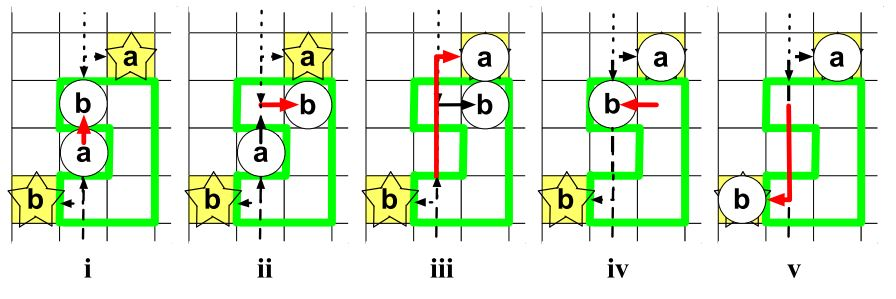
\includegraphics[width=\linewidth]{graphics/mappblank}
	\label{fig:mappblank}
	\caption{Example of how MAPP works (\cite{wang2011mapp})}
\end{figure}

In comparison to FAR and WHCA*, MAPP excels in having high completeness at 92\%--99.7\%, compared to FAR (81.87\%) and WHCA* (80.87\%). Speed-wise, MAPP is comparable to WHCA* and 10 times slower than FAR  but in scenarios where MAPP has $\Omega$ paths, MAPP is 2.18 times slower than FAR and 4.8--5.2 times faster than WHCA*.



\begin{figure}[H]
	\centering
	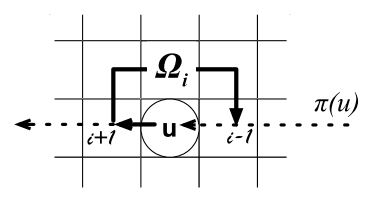
\includegraphics[width=0.4\linewidth]{graphics/omegapath}
	\label{fig:omegapath}
	\caption{An example of an alternate path, $\Omega$ (\cite{wang2011mapp})}
\end{figure}


\section{Optimal multi-agent pathfinding algorithms} \label{sec:optimal}
Optimal MAPF algorithms usually use a coupled approach also known as centralized approach. A coupled approach finds paths for all agents at once. 




Here we look at multi-agent pathfinding algorithms which aim to find the optimal solution based on some objective function. The objective function will be noted per algorithm. Our main aim is to determine the benefits and downsides of each algorithm.


Coupled approach: All agents at one! A* ICTS

\cite{krontiris2013feasibility} looked at the feasibility.

\subsection{Centralized A*}
Centralized A* is exponential in the number of agents $O(n^k)$

There are a number of algorithms based on Centralized A*, 

One variant of is an algorithm called enhanced partial A* expansion (EPEA*). The original algorithm \cite{yoshizumi2000partial}. An improvement on PEA* is EPEA* (\cite{felner2012partial}, \cite{goldenberg2014enhanced}).

Another variant is M*.

Independence Detection and Operator Decomposition provides an exponential speed up to Centralized A* as it reduces the number of agents being processed, more details about ID in Section~\ref{sec:od} and OD in Section~\ref{sec:od}.

\cite{ferner2013odrm} improves on M* by applying operator decomposition.

\subsection{Conflict based search} \label{sec:cbs}
The conflict-based search algorithm (\cite{sharon2015conflict}) relies on building a binary tree known as a  \textit{constraint tree} (CT). Each node in the CT describes a set of constraints, a solution and the cost of this solution. A constraint prohibits an agent $a$ from being at node $n$ at timestep $t$, in the form of $\langle a, n, t \rangle$.

A node in the CT is processed by finding the shortest path for each agent to their goal making sure to satisfy the constraints described by the node. If this path is not valid and a collision has occurred between two agents: $a_1, a_2$ then CBS branches and adds two successor nodes. Both successor nodes inherit the constraints of the parent node. Additionally the left successor will adds a new constraint $\langle a_1, n, t \rangle$ while the right node will add the constraint $\langle a_2, n, t \rangle$. CBS is optimal as it chooses the node to expand searching the constraint tree for the node with the lowest cost.

As CBS branches at every conflict, it is exponential in the number of conflicts. In comparison to EPEA*, CBS performed worse in maps with open spaces where sets of agents may be \textit{strongly coupled}, that is they frequent have a high rate of path conflicts between one another. On the other hand CBS was found to perform better in maps with bottlenecks, where A* would 


CBS is exponential in the number of conflicts In comparison to ICTS and A* CBS was found to be best in maps with bottlenecks (Fig.~\ref{cbsresults1}).

A bounded-suboptimal variant of CBS, ECBS features \cite{barer2014suboptimal} \textbf{TODO} Recently iECBS expanded on this with the use of highways and  \cite{cohen2016improved}.

\begin{figure}[!htb]
	\centering \tiny
	\begin{minipage}{0.4\textwidth}
	\centering
	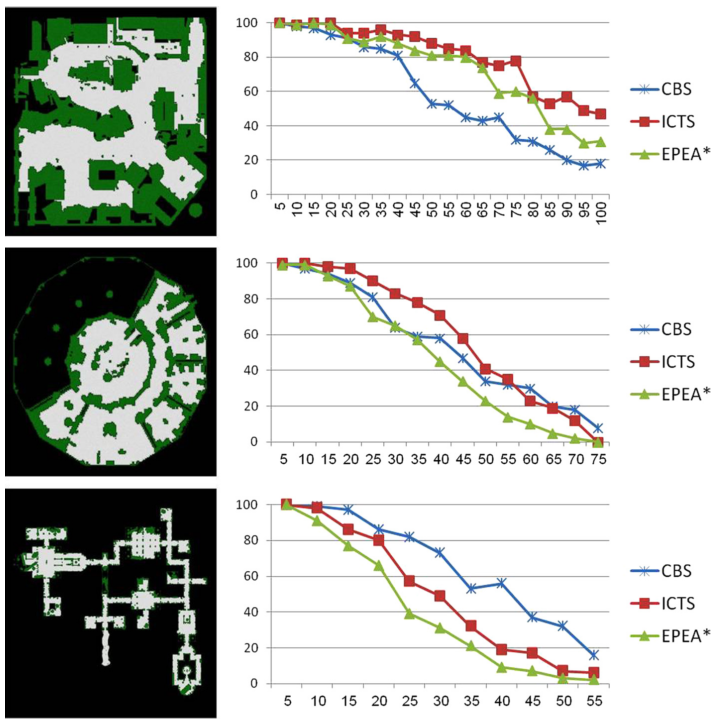
\includegraphics[width=\linewidth]{graphics/cbsresults1}
	\caption{A Small Region of a Kiva Layout (\cite{sharon2015conflict}). Picking stations located on the left and storage pods laid out in rows.}
	\label{cbsresults1}
	\end{minipage}
	\begin{minipage}{0.4\linewidth}
		\centering
	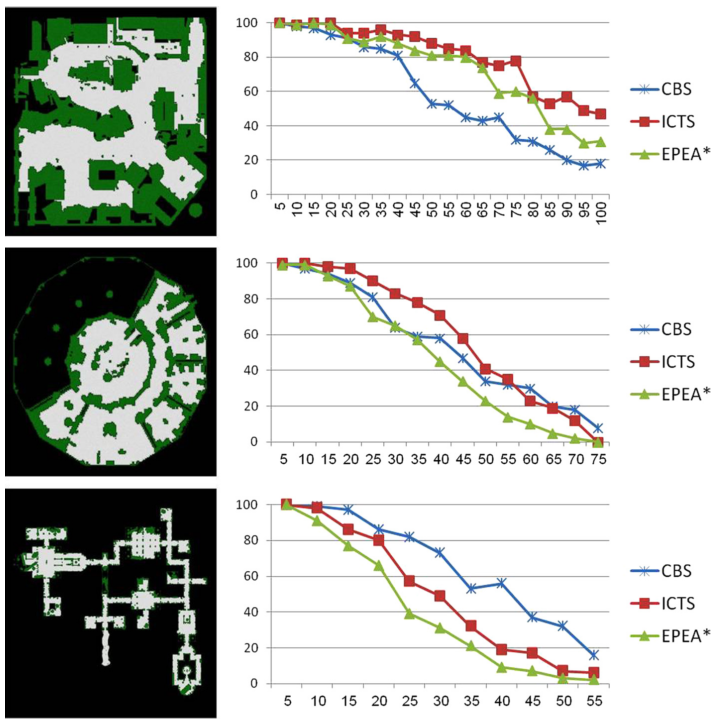
\includegraphics[width=\linewidth]{graphics/cbsresults1}
	\caption{A Small Region of a Kiva Layout (\cite{sharon2015conflict}). Picking stations located on the left and storage pods laid out in rows.}
	\label{cbsresults2}
	\end{minipage}
\end{figure}

Here CBS was compared against ICTS, EPEA*.

\subsection{Increasing Cost Search Tree}
This section describes the Increasing Cost Search Tree (ICTS) an optimal, complete MAPF algorithm (\cite{sharon2011increasing}). The ICTS algorithm generates a tree known as an \textit{increasing cost tree} (Figure~\ref{fig:increasingcosttree}). Each node in the tree describes a cost $C$ for each agent $[C_1,\dots,C_k]$. ICTS finds a valid solution when every agent $a_i$ is conflict-free and it generates these paths based off the cost described in the node by exploring all paths which are equal to $C_i$.  To build the tree, the root starts containing the an optimal cost disregarding any conflicts for each agent. When it does not find a valid solution, the algorithm will branch and generate $k$ successors, one for each agents. In each of the successors, the cost of $i$ will increment e.g. for successor 2: $[C_1,C_{2}+1,\dots,C_k]$. By exploring the tree in breadth-first manner, ICTS ends up with an optimal solution.

\begin{figure}[!htb]
	\centering
	\centering
	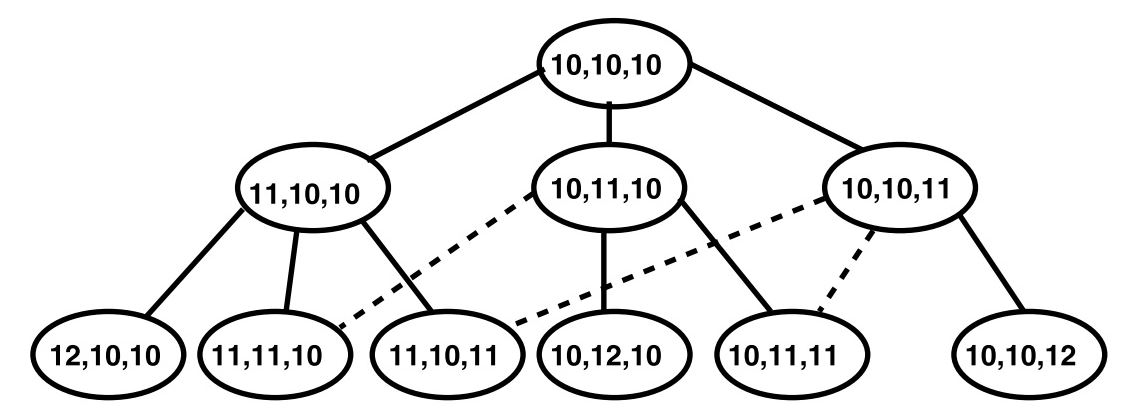
\includegraphics[width=0.9\linewidth]{graphics/ictstree}
	\caption{ICT for three agents (\cite{sharon2011increasing})}
	\label{fig:increasingcosttree}
\end{figure}

The ICT grows exponentially in $\Delta$, where delta is the difference between the optimal collision-free cost and the optimal cost which ignores collision (the root node). Hence the downfall of ICTS is an environment with many conflicts occurs or it is costly to resolve the conflicts, thus having a large $\Delta$. In comparison to $A*$ which is exponential in $k$, ICTS is exponential in $\Delta$ so it benefits most on open maps with many agents.

%\subsection{Integer Linear Programming}
%Integer Linear Programming (ILP) is an optimization technique. It looks at an objective function subject to a list of constraints and finds the optimal solution for each variable.
%
%\subsection{ILP (combined target-assignment and pathfinding)}
%\cite{ma2016optimal} covers the use of Network Flow, More details about the use of ILP is in Section~\ref{sec:tapf}.
%
%where agents are anonymous. 
%
%reduction to the integer multi- commodity flow problem on a time-expanded network.
%
%\cite{yu2016optimal} takes a Network Flow approach. The solver uses the branch-and-bound algorithm. Anytime approach.

%\subsection{ILP (Network Flow)}
%\cite{yu2013multi} connects multi-agent path planning on graphs (roadmaps) to network flow problems, showing that the former can be reduced to the latter, therefore enabling the application of combinatorial network flow algorithms, as well as general linear program techniques, to multiagent path planning problems on graphs.
%
%\cite{yu2016optimal} looks at Complete Algorithms and Effective Heuristics.
%
%\cite{yu2015optimal} looks at the Structure and Computational Complexity.

\subsection{Combined-target assignment and pathfinding} \label{sec:tapf}
This section describes the work by \cite{ma2016optimal}, which looks at developing MAPF algorithms for autonomous warehouse robots, they call this a combined assignment and pathfinding (TAPF) problem. Importantly the difference between a MAPF problem and a TAPF problem is that:

\begin{itemize}
	\item Agents are split into teams and a team of $k$ agents will have $k$ goal locations
	\item Agents are anonymous: any agent in a team can be assigned to a goal location
\end{itemize}

An important property is that anonymous MAPF problems are usually solved in polynomial time. This paper describes two algorithms which are made to solve the TAPF problem. Both of these at the low-level uses a a min-cost max-flow algorithm.

\subsubsection{CBM}
Conflict-based min-cost flow (CBM)  hierarchical algorithm, as the name describes uses CBS (\ref{sec:cbs}) at the high-level and  on the low-level.

\subsubsection{ILP (TAPF)}
Similar to CBM but instead of using CBS at the high level an ILP-based TAPF solver is used at the low-level. This ILP solver is based off the work by (\cite{yu2013multi}) and uses a network-flow approach. Results found that this solver performed worse than the ILP MAPF solver in runtime and success rate but won in makespan.

CBM is applied to Kiva Systems which is the motivation behind formulating the TAPF problem. Their problem instances for Kiva Systems contain 420 drive units moving to 7 picking stations, the total warehouse size was not stated. Results suggested that CBM was performed well enough to be used in real-world applications of Kiva systems, with an 80\% success rate, mean makespan of 63.83 seconds and mean running time of 91.61 seconds. Importantly the results beat that of bounded suboptimal MAPF algorithms which were designed for Kiva systems.

\section{Independence detection and Operator decomposition} \label{sec:generalimprovements}
Here we two techniques which can be applied to most MAPF algorithms.

\textbf{Independence detection}. Independence detection (ID) finds independent groups of agents where it can be proven that these two groups will not be in conflict. These groups are split and treated as seperate subproblems. Importantly this reduces the number of agents and provides an exponential speed up for A* and a polynomial speedup for many non-A* based algorithms.

\textbf{Operator decomposition}. Operator decomposition (OD) reduces the branching factor by performs one agents action at a time as oppose to an operator applying to every agent simultaneously. OD gives a much deeper tree but with a much smaller branching factor. At every $k$ levels in the tree we get an equivalent state where OD would not be used and hence the branching factor can be seen as $a$ instead of $a^k$ where $a$ is the number of possible actions and $k$ is the number of agents.

\cite{standley2010finding} found that OD had larger benefits and scaled better than ID. Regardless they can both be used.

\subsection{Independence detection} \label{sec:id}
\cite{standley2010finding} Independence detection (ID) allowed the paths of groups of agents to be computed independently, without sacrificing optimality 

%\textbf{Standley (Standley 2010) presented (= ?V independence detection (ID) framework. ID partitions the problem into smaller independent subproblems, if possi- ble, and solves each problem separately. Standley also intro- duced operator decomposition (OD) which considers mov- ing a single agent at a time. OD reduces the branching fac- tor at the cost of increasing the depth of the solution in the search tree.}

\subsection{Operator decomposition} \label{sec:od}
\cite{standley2010finding} Operator decomposition (OD) is used to reduce the branching factor of the MAPF algorithms.
x
\section{Discussion} \label{sec:discussion}

\begin{table}
	\centering
	\small
	\begin{tabular}{ l c c c c c p{2.3cm}}
		
		\textbf{Name} & \textbf{BSV} & \textbf{Complete} & \textbf{Complexity} & \textbf{SQ} & \textbf{KS} & \textbf{Comparison} \\
		\hline
		\multicolumn{7}{l}{\textbf{Optimal}} \\
		\hline
		CBS 				& N & Y & Exp conflicts & Opt & Y & ICTS, EPEA* \\
		Centralized A* 		& Y & Y & Exp agents & Opt & N & ??? \\
		ICTS 				& Y & Y & Exp $\Delta$ & Opt & N & A*, A*+OD \\
		ILP	(NF)			& Y & Y & Exp conflicts & Opt & Y & CBS \\
		ILP	(TAPF)			& N & Y & Exp conflicts & Opt & Y & ILP (NF), IPL (TAPF) \\
		CBM 				& N & Y & Exp conflicts & Opt & Y & ILP (NF), IPL (TAPF) \\
		\hline
		\multicolumn{7}{l}{\textbf{Suboptimal}} \\
		\hline
		FAR  				& N & N & Poly & Sub Opt & N & \\
		MAPP 				& Y & Y & Poly & Sub Opt & N & WHCA*, FAR \\
		WHCA* 				& N & N & Poly & Sub Opt & N & \\
	\end{tabular}

	\caption{Table comparing the stated algorithms and their properties. \textbf{SQ}: solution quality. \textbf{BSV}: Does the algorithm have a bounded-suboptimal variant. \textbf{Complexity}: Runtime complexity. \textbf{KS}: has the algorithm been applied to Kiva systems. \textbf{Comparision}: the algorithms used for benchmark testing.}
	\label{table:comparison}
\end{table}


Most optimal algorithms improve scalability by relaxing the solution quality and creating a bounded-suboptimal variant. or defining a special case of the MAPF problem, TAPF.


In regards to Kiva systems, results find that the biggest winner by a large margin is CBM. CBM is an optimal, complete algorithm which wins over even the bounded-suboptimal variants of CBS. Importantly CBM defines a TAPF problem where agents are anonymous.

With suboptimal algorithms, none were applied to Kiva systems. It would be useful to see the relative makespans of the system for a suboptimal solution, compared to that of algorithms such as CBM or CBS.

Lastly, we find that the downtime of the solution is overlooked and instead makespan is used as the objective. Commonly, including more robots in the simulation will fulfill the down-time but this has an exponential effect on the complexity of optimal algorithms. The relation between the number of agents and tradeoffs between runtime and downtime may find some pitfalls of an optimal solution. 

Ultimately We should study these algorithm in the warehouse environment. Besides CBS and ILP (TAPF), other algorithms have not been compared against one another. Our research focuses on the area of ILP.


\bibliographystyle{dcu}
\bibliography{bibliography}
	
\end{document}
